% !TEX root = EUDAQUserManual.tex
\section{Running EUDAQ}
This section will describe running the DAQ system, mainly from the point of view of the
EUDET JRA1 Pixel Telescope\cite{eudet2009} with a \gls{DUT}, although most of it should
also be applicable to the DAQ in general, even without the telescope.

All executable programs from the different subdirectories are placed inside the \texttt{bin} subdirectory,
and should be run from here.

They should all accept a \texttt{-h} (or \texttt{--help}) command-line parameter,
which will provide a summary of the different command-line options that can be used.

\subsection{Preparation}
Some preparation is needed to make sure the environment is set up correctly and
the necessary TCP ports are not blocked before the DAQ can run properly.

\subsubsection{Directories}
The DAQ expects two directories to exist, that it will use to store data files and log files.
They need not be real directories -- they can be symbolic links to other directories
if you don't want to store the files inside the EUDAQ installation.

First, inside the \texttt{eudaq} directory, there should be a directory (or symbolic link) called \texttt{data}.
This will contain the data files written by the Data Collector, as well as a file containing the last run number,
so that it will continue incrementing even when the DAQ is restarted.

Secondly, there should be a directory (or symbolic link) called \texttt{logs}.
This will be used by the Log Collector to store log files containing all the log messages received.

\subsubsection{Firewall}
The different processes communicate between themselves using TCP/IP sockets.
If a firewall is running, it may block these connections,
especially if the processes are running on different computers.
If all the processes will be run from the same computer,
then it is probably not necessary to do anything.
If a port is blocked, you will see an error message similar to the following
when attempting to start some programs:
\begin{listing}[]
Are you sure the server is running? - Error 61 connecting to localhost:44000: Connection refused
\end{listing}

The ports used may be configured on the command line, but the default values used are:
\begin{description}

\ttitem{44000}
This is the port used to send commands from the Run Control.

\ttitem{44001}
This port is used to send data from the producers to the Data Collector.

\ttitem{44002}
This port is used to send log messages from all processes to the Log Collector.

\end{description}

If processes will be run on different computers,
then these ports should be opened up in the firewall.
The method for doing this depends on the Operating System used,
and is outside the scope of this manual.

\subsubsection{Environment}
When a process connects to the Run Control, it must be told what addresses to use
to connect to the Log Collector and (if it is a Producer) to the Data Collector.
The Run Control will ask the Log and Data Collectors what address to report,
and these processes therefore need a way to determine what address they are listening on.
There is no completely fool-proof way of determining this,
so they look at the environment variable \texttt{\$HOSTNAME}.

Usually this should be the DNS name of the machine it is running on, but in some cases it may not work correctly.
If this is the case, it may be necessary to set this variable manually, either to the real host name,
or the machine's IP address, or (if all the processes will be run on the same computer) it can be set to \texttt{localhost}.

Depending on the command shell used, the command to do this should be either
``\inline[mybash]{export HOSTNAME=name}'' (for bash-like shells)
or ``\inline[csh]{setenv HOSTNAME name}'' (for csh-like shells),
where \texttt{name} is the name to use.

\subsubsection{TLU permissions}\label{sec:TLUperm}
If you are not using a TLU, or not running on Linux, you may skip this part.

On many Linux distributions, the device node used to communicate over the USB bus is only
accessible by the user \texttt{root} by default.

To have the system set the correct permissions when a \gls{TLU} is
connected, you need to add a \texttt{udev} rule: as \textrm{root}
user, create the file \texttt{/etc/udev/rules.d/54-tlu.rules} and add
the following lines:

\begin{listing}
# for Red Hat, e.g. SL5
SYSFS{idVendor}=="165d", SYSFS{idProduct}=="0001", GROUP="NOROOTUSB", MODE="0666"
\end{listing}

if you are using a Red~Hat-based distribution (such as Scientific
Linux) or:

\begin{listing}
# for Debian
ACTION=="add", DRIVERS=="?*",  ATTR{idVendor}=="165d", ATTR{idProduct}=="0001",  MODE="0666"
\end{listing}

in case you are using a debian-based distribution such as Ubuntu.

After replugging the {TLU}, the device should be accessible by
all users.


\subsection{Processes}
The DAQ system is made up of a number of different processes that may all be run on the same,
or on different computers. They are each described below.

\subsubsection{Run Control}
There are two versions of the Run Control -- a text-based version, and a graphical version (see \autoref{fig:RunControl}).
The graphical version is preferred, since it is the most used, and therefore the most tested and complete.
The executable is called \texttt{euRun.exe}, or on Mac OS X it is an application bundle called \texttt{euRun.app}.
The text-based version can be useful for testing, the executable is \texttt{TestRunControl.exe}.

\begin{figure}[htb]
  \begin{center}
    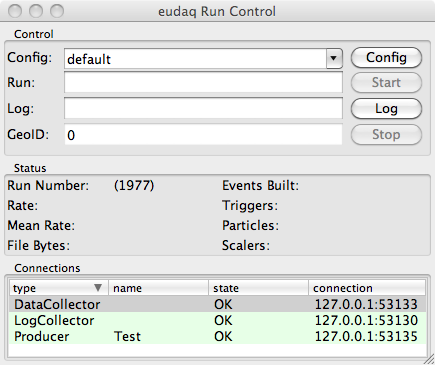
\includegraphics[width=0.6\textwidth]{src/images/RunControl}
    \caption{The Run Control graphical user interface.}
    \label{fig:RunControl}
  \end{center}
\end{figure}

Normally no command-line options should be needed, but it can be told to listen on a non-standard port,
(e.g. to run two copies on the same machine), with the \texttt{-a \param{port}} option:
\begin{listing}[mybash]
$[./euRun.app/Contents/MacOS/euRun]$ -a 3000
\end{listing}

This example is for Mac OS X, where the executable is inside an application bundle,
on other architectures it will be just \texttt{euRun.exe}.
Note also that it is not recommended to run two copies of the DAQ simultaneously,
since it becomes difficult to keep them completely separate as the Log and Data Collectors
must also be run on different ports.

\subsubsection{Log Collector}
Running the Log Collector is optional. If it is run, then all log messages generated by all other processes
in the DAQ will be collected in one central location.

\begin{figure}[htb]
  \begin{center}
    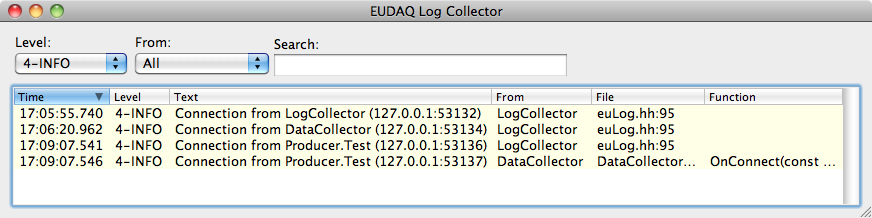
\includegraphics[width=\textwidth]{src/images/LogCollector}
    \caption{The Log Collector graphical user interface.}
    \label{fig:LogCollector}
  \end{center}
\end{figure}

Like the Run Control, there are also two versions of the Log Collector.
The graphical version is called \texttt{euLog.exe}, or \texttt{euLog.app} on Mac OS X,
and the text-based version is called \texttt{TestLogCollector.exe}.

If it is being run on the same machine as the Run Control, it should not need any command-line options.
However, if it is run on a different machine, it must be told on which machine the Run Control is running,
using the \texttt{-r \param{hostname}} option, e.g.:
\begin{listing}[mybash]
$[./euLog.exe]$ -r eudetmac001.cern.ch
\end{listing}

It may also be told to listen on a non-standard port, using the \texttt{-a \param{port}} option, similar to the Run Control.

\subsubsection{Data Collector}
The Data Collector is the process that collects all the raw data from the Producers,
merges all the connected incoming streams into a single data stream, and writes it to file.

Like the Log Collector, it should be told where to connect to the Run Control if it is not running on the same machine,
and it may also be told to listen on a non-standard port, with the \texttt{-r} and \texttt{-a} options respectively, for example:
\begin{listing}[mybash]
$[./TestDataCollector.exe]$ -r eudet -a tcp://55001
\end{listing}

It is also possible to run multiple Data Collector instances within
one EUDAQ session. This can be useful to reduce network traffic and
e.g. write the output of one producer to a locally attached disk. When running
several Data Collectors simultaneously, Run Controls assigns a
Producer to a Data Collector by name: if the name of a Data Collector
matches that of a Producer, the latter will be given the address and
port of the former. There can be only one instance of an \emph{unnamed} Data
Collector which serves as the default for any non-matching Producer;
if no unnamed Data Collector is present, the first one connecting will
serve as the default.

The name of a Data Collector can be set with the
\texttt{-n} option, for example:
\begin{listing}[mybash]
$[./TestDataCollector.exe]$ -n myproducer
\end{listing}

Should you wish to run several instances of the Data Collector on one
machine, you need to make sure that they listen to different addresses
using the \texttt{-a} option as described above. Furthermore, you need
to make each Data Collector write to a different file by including the
\texttt{FilePattern} option in the corresponding section of your
configuration file (also see section \ref{sec:ConfigFiles}):

\begin{listing}[conf]
[DataCollector.myproducer]
FilePattern = "../data/run$6R_myproducer$X"
\end{listing}

\subsubsection{TestProducer}
For testing purposes, you may use the Test Producer.
This works similarly to a real producer, but does not talk to any real hardware,
instead providing a menu for the user to manually send events
(or see the ExampleProducer, below).

\subsubsection{ExampleProducer}
The ExampleProducer was written to illustrate the writing of a new Producer (see \autoref{sec:Producers}).
However, it will actually generate some example data, and so can also be used for testing purposes.
It works more like a real Producer than the TestProducer,
in that it does not require user intervention to generate each trigger,
and the data generated emulates a simple (but realistic) sensor,
and can be properly converted, and therefore displayed in the Monitor.

\subsubsection{TLUProducer}
If you do not have a \gls{TLU} in your setup, you may skip this part.
Otherwise you should run a TLUProducer, which will configure the \gls{TLU},
and read out the timestamps and send them to the Data Collector.

On the computer with the \gls{TLU} connected, start the \texttt{TLUProducer.exe} program.
If this is not the same machine as the Run Control,
use the \texttt{-r} option as for the Data and Log Collectors.
For example:
\begin{listing}[mybash]
$[./TLUProducer.exe]$ -r eudet.unige.ch:3000
\end{listing}

If the TLUProducer fails to start, make sure the permissions are set up correctly (see \autoref{sec:TLUperm}).

\subsubsection{EUDRBProducer}
The \gls{EUDRB} boards are used to read out the telescope sensors.
The \gls{EUDRB} Producer is designed to run on a Motorola MVME6100 single board computer,
using the Tundra TSI148 VME bridge for communication with the \glspl{EUDRB}.

If more than one EUDRBProducer is to be run, they must all have different names.
The name can be set with the \texttt{-n \param{name}} option.

As with the other processes, the address of the Run Control should be set with the \texttt{-r} option.
An example is shown below:
\begin{listing}[mybash]
$[./EUDRBProducer.exe]$ -n EUDRB2 -r 192.168.1.1
\end{listing}

\subsubsection{Other Producer(s)}
If you have a producer for your own hardware (see \autoref{sec:Producers}),
it should also have an option to set the address of the Run Control.

\subsubsection{OnlineMon}

The OnlineMon reads the data file written by the Data Collector,
and generates several Root histograms that can be useful for online monitoring.
Since it reads the native data file directly, it must be run on the
same machine as the Data Collector.

\begin{figure}[htb]
  \begin{center}
    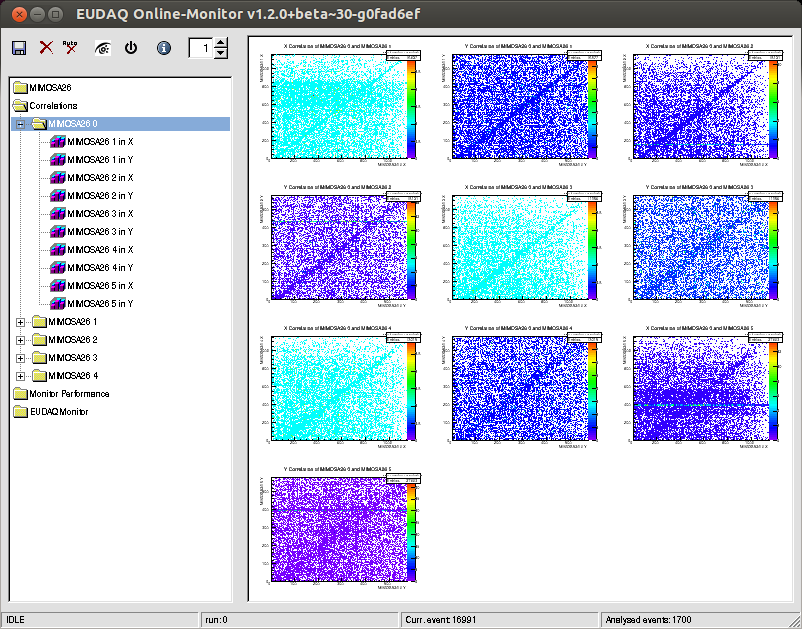
\includegraphics[width=0.8\textwidth]{src/images/OnlineMonCorrelations}
    \caption{The OnlineMon showing correlation plots between different
      Mimosa26 planes of the EUDET telescope.}
    \label{fig:OnlineMonPlots}
  \end{center}
\end{figure}


The OnlineMon can be run in one of two modes: online or offline.
In online mode, it connects to the RunControl, so it will know when new runs are started,
and it will automatically open each new data file as it is created.
In offline mode, there is no RunControl,
and it only analyses the data file it is given on the command line. 
An example command line is:
\begin{listing}[mybash]
$[./OnlineMon.exe]$ -f 5432
\end{listing}

This will run it in offline mode, opening the file corresponding to run 5432
(alternatively, the full path to a file may be given).
To run it in online mode, simply omit the \texttt{-f} option,
then the \texttt{-r} option may be used if the RunControl
is running on a different computer or using a non-standard port.

\subsubsection{Python Interface and Wrapper for Core EUDAQ Components}
\label{sssec:pywrapper}
A Python interface is provided for selected EUDAQ components:
RunControl, DataCollector and a Producer, that can be extended on the
Python side. The interface is realized through the \texttt{ctypes}
package that is part of every standard Python installation and
requires the \texttt{numpy} Python package to be installed. The
interface code for all components is located in the
\texttt{main/python} directory.

To use the interface and access the components as Python objects, the
wrapper must be loaded inside your Python script:

\begin{listing}[python]
  #!/usr/bin/env python2 
  execfile('PyEUDAQWrapper.py') # load ctypes wrapper

  prc = PyRunControl() # start run control with default settings
  # wait for more than one active connection to appear
  while prc.NumConnections < 2:
      sleep(1)
  prc.Configure("ExampleConfig") # load configuration file
  while not prc.AllOk:
      sleep(1) # sleep while waiting for all connected producers
  prc.StartRun()
\end{listing}

This little scripts creates a RunControl instance, sends a
configuration to all connected producers, waits for their reply, and
starts a new run. Several more extensive examples for using Python
with EUDAQ are located in the \texttt{python} directory in the main
EUDAQ directory.


\subsection{Running the DAQ}
To start the DAQ, all the necessary processes must be started in the correct order.
The first process must be the Run Control,
since all other processes will attempt to connect to it when they start up.
Then it is recommended to start the Log Collector,
since any log messages it receives may be useful
to help with debugging in case everything does not start as expected.
Next, the Data Collector should be started.
Finally all the Producers, and if needed, the RootMonitor.

\subsubsection{STARTRUN}\label{sec:STARTRUN}
The \texttt{STARTRUN} file, in the main \texttt{eudaq} directory
(as opposed to the \texttt{bin} subdirectory where the executables exist),
is a shell script that can be customized to load the appropriate processes for running the DAQ.
This allows you to start all the processes necessary with a single command.
If starting processes on other computers via SSH,
it is recommended to set up SSH keys so that the processes may be started without having to type a password.

In the future the \texttt{STARTRUN} script may be replaced with a more intelligent version
that uses a configuration file generated by the config script to decide what to load.

\subsubsection{Controlling the DAQ}
Once all the processes have been started, the DAQ can be configured, and runs may be started and stopped
using the Run Control (see \autoref{fig:RunControl}).

First the appropriate configuration should be selected from the drop-down list
(see \autoref{sec:ConfigFiles} for creating and editing configurations),
and the \texttt{GeoID} should be verified (see \autoref{sec:GeoID}), before continuing.

Then the \texttt{Config} button can be pressed,
which will send a configuration command
(with the contents of the selected configuration file) to all connected processes.
The full contents of the configuration file will also be stored
in the \gls{BORE} of the data file,
so that this information is always available along with the data.

Once all connected processes are fully configured, a run may be started, by pressing the \texttt{Start} button.
Whatever text is in the corresponding text box when the button is pressed
will be stored as a comment in the data file.
This can be used to help identify the different runs later.

Once a run is completed, it may be stopped by pressing the \texttt{Stop} button.
Runs will also stop and restart automatically when the data file reaches a threshold in size
(by default this is 1~GB).
This is because there is a file size limit of 2~GB for storage on the GRID,
and the processed files can grow bigger than the original native files.
The threshold size for restarting a run may be configured in the config file (see \autoref{sec:ConfigFiles}).

At any point a message may be sent to the log file by filling in the \texttt{Log} text box and pressing the corresponding button.
The text should appear in the LogCollector window, and will be stored in the log file for later access.

Once the run is stopped, the system may be reconfigured with a different configuration, or another run may be started.

\subsubsection{Config Files}\label{sec:ConfigFiles}
The \texttt{Config} drop-down in the Run Control is populated from the files in the \texttt{config} subdirectory.
These are just text files in a specific format, containing name-value pairs separated into different sections.
See \autoref{sec:ExampleConfig} for an example file.

Any text from a \texttt{\#} character until the end of the line is treated as a comment, and
ignored.  Each section in the config file is delimited by a name in square brackets
(e.g. \verb@[RunControl]@).  The name represents the type of process to which it applies; if there
are several such processes, then they can be differentiated by including the name after a period
(e.g. \verb@[Producer.Example]@).  Within each section, any number of parameters may be specified,
in the form \mbox{\texttt{Name = Value}}.  It is then up to the individual processes how these
parameters are interpreted.

The entire contents of the config file will be sent to all processes during the configuration, and
each process will have the appropriate section selected.  The file will also be attached to the
\gls{BORE}, so that it is available with the data later, even if the original config file is
modified or deleted.

\subsubsection{GeoID}\label{sec:GeoID}
The GeoID is a number representing the physical positioning of the telescope and DUT(s).
Each time a change is made to the telescope layout, this number should be incremented.
To change the number, double-click on it, and a window will appear with the new value.
By default it will increment the old value by one, so normally you should just click \texttt{OK},
but if necessary you may edit the value first.

The GeoID is inserted into the config file when it is sent, so it is also stored in the data file,
and will be used to select the correct GEAR file for alignment during the data analysis stage.

\subsection{Other Utilities}
There are a number of other utilities available that are not needed for running the DAQ,
but can be useful for other tasks such as debugging.
The executables are all located in the \texttt{bin} subdirectory.
They should all accept a help (\texttt{-h} or \texttt{--help}) option,
to print a summary of the available options.

\subsubsection{TLUControl}
The \texttt{TLUControl.exe} program is a standalone program for running the TLU without using the
full DAQ. The most commonly used parameters are shown below. For each option, the short (preceeded
by one dash) and the long (preceeded by two dashes) option names are shown (only one of the two
forms should be used for each option, but long and short options can be mixed together on the
command line), along with any parameters and their default value that will be used if the option is
not specified.

\begin{description}
\ttitem{-d --dutmask \param{mask = 0}}
The DUT mask; this defines which DUT connections are activated.  It is a bit-mask, so 1 means
connector 0, 2 means connector 1, etc..

\ttitem{-a --andmask \param{mask = 255}}
The AND mask; this defines which external trigger inputs are activated. It is a bit-mask, so 1
means channel 0, 2 means channel 1, etc.. The specified channels are ANDed together, and used to
generate a trigger signal.

\ttitem{-t --trigger \param{msecs = 0}}
Internal trigger period.  If non-zero, the \gls{TLU} will generate internal triggers with the
specified period in milliseconds. If set to zero, the internal trigger is off.

\ttitem{-i --dutinputs \param{values = ""}}
Input mode select. A sequence of comma-separated strings specifying which connectors to use for the
DUT inputs. Valid values are \texttt{RJ45}, \texttt{LEMO}, \texttt{HDMI}, and \texttt{NONE}.

\ttitem{-u --wait-for-user}
Pause the program after the \gls{TLU} is configured, before starting triggers. The default is to not
wait for the user.
\end{description}

Other parameters available are as follows:

\begin{description}
\ttitem{-o --ormask \param{mask = 0}}
The OR mask; this defines which external trigger inputs are activated. It is a bit-mask, so 1
means channel 0, 2 means channel 1, etc.. The specified channels are ORed together, and used to
generate a trigger signal.

\ttitem{-v --vetomask \param{mask = 0}}
The VETO mask; this defines which external trigger inputs are activated. It is a bit-mask, so 1
means channel 0, 2 means channel 1, etc.. The specified channels are used to veto the generation
of a trigger if they are active.

\ttitem{-w --wait \param{ms = 1000}}
Wait time. This is the time to wait between updates.

\ttitem{-n --notimestamp}
Indicates that the timestamp buffer should not be read out.

\ttitem{-q --quit}
Quit the program after configuring the TLU.

\ttitem{-s --save-file \param{filename = ""}}
     The filename to save trigger numbers and timestamps

\ttitem{-p --strobeperiod \param{cycles = 1000}}
Period for timing strobe (in \gls{TLU} clock cycles).

\ttitem{-l --strobelength \param{cycles = 100}}
Length of `on' time for timing strobe (in \gls{TLU} clock cycles).

\ttitem{-b --dutveto \param{mask = 0}}
Mask for enabling veto of triggers (`backpressure') by rasing DUT\_CLK.

\ttitem{-hm --handshakemode \param{nohandshake = 0}}
In this mode the TLU issues a fixed-length pulse on the trigger line (0 = no handshake).

\ttitem{-pw --powervctrl \param{mV = 800}}
[obsolete but provided for backward compatibility, please use \texttt{-pv}] Sets the Vcntl control
voltage to all PMTs. The range of values is between 0 and 1000 (or 0 and 2000 if the \gls{TLU} has
been modified by cutting \texttt{LC1} and jumpering \texttt{LO1} on the PMT Supply Daughterboard and
specifying the \texttt{-pm 1} option).

\ttitem{-pv --pmtvcntl \param{mV = 800}}
Sets the Vcntl control voltage to all PMTs (see option \texttt{-pw} for more details). Will override
the value of \texttt{-pw} if it is specified. If neither \texttt{-pw} or \texttt{-pv} is specified,
the default value will be used (and can be overridden on an individual PMT basis).

\ttitem{-p1 --pmtvcntl1 \param{mV}}
Sets the PMT Vcntl voltage for PMT1 (Chan 0) only. If not specified, the default or values specified
by \texttt{-pw} or \texttt{-pv} (which will override \texttt{-pw}) is used.

\ttitem{-p2 --pmtvcntl2 \param{mV}}
Sets the PMT Vcntl voltage for PMT2 (Chan 1) only. If not specified, the default or values specified
by \texttt{-pw} or \texttt{-pv} (which will override \texttt{-pw}) is used.

\ttitem{-p3 --pmtvcntl3 \param{mV}}
Sets the PMT Vcntl voltage for PMT3 (Chan 2) only. If not specified, the default or values specified
by \texttt{-pw} or \texttt{-pv} (which will override \texttt{-pw}) is used.

\ttitem{-p4 --pmtvcntl4 \param{mV}}
Sets the PMT Vcntl voltage for PMT4 (Chan 3) only. If not specified, the default or values specified
by \texttt{-pw} or \texttt{-pv} (which will override \texttt{-pw}) is used.

\ttitem{-pm --pmtvcntlmod \param{value = 0}}
Specifies whether the TLU PMT Supply Daughtercard is modified (\texttt{LC1} cut and \texttt{LO1}
jumpered) or not.  A \param{value} of 0 specifies that it is unmodified (and thus the Vcntl range is
from 0mV to 1000mV), and a \param{value} of 1 specifies that the \gls{TLU} is modified (and thus the
Vcntl range is from 0mV to 2000mV).  This feature is to accomodate newer Hamamatsu PMT models
(e.g. H10721) that require a control voltage range of, for instance, 500mV to 1100mV that are being
used in place of the older (discontinued, but what the \gls{TLU} was designed to accomodate and
control) models that required a control voltage of between 250mV and 900mV.

\ttitem{-f --bitfile \param{filename = ""}}
The bitfile containing the TLU firmware to be loaded.

\ttitem{-e --error-handler \param{value = 2}}
Error handler setting. Setting to 0 indicates the program should abort on an error. Setting it to a
value greater than 0 indicates the number of tries that should be attempted before generating an
exception.

\ttitem{-r --fwversion \param{value = 0}}
Specifies the firmware version to load (setting to 0 indicates the version should be chosen automatically).

\ttitem{-z --trace-file \param{filename = ""}}
The filename to save a trace of all USB accesses. Prepend a dash (`\texttt{-}') to output errors
only, or a plus (`\texttt{+}') for all data (including block transfers).
\end{description}

An example use of the command is shown below:

\begin{listing}[mybash]
$[./TLUControl.exe]$ -t 200 -d 3 -i LEMO,RJ45 -u
Using options:
TLU version = 0 (auto)
Bit file name = '' (auto)
Trigger interval = 200 ms (5 Hz)
DUT Mask  = 0x03 (3)
Veto Mask = 0x00 (0)
And Mask  = 0xff (255)
Or Mask   = 0x00 (0)
DUT inputs = LEMO,RJ45
Strobe period = 0x0003e8 (1000)
Strobe length = 0x000064 (100)
Enable DUT Veto = 0x00 (0)
Save file = '' (none)

TLU Version = v0.2c
TLU Serial number = 0x062b (1579)
Firmware file = TLU2_Toplevel.bit
Firmware version = 65
Library version = 65

Press enter to start triggers.

TLU Started!

Status:    20,00,--,--,--,-- (0,0)
Scalers:   0, 0, 0, 0
Particles: 2
Triggers:  0
Entries:   0
TS errors: 0, 0 (redundancy, re-read)
Timestamp: 0x8d768 (579432) = 0.00150891
Time: 0.009 s, Freq: 0 Hz, Average: 0 Hz

        0, 0x27fb479 (41923705) = 0.109174, diff=41923705
        1, 0x7139ab9 (118725305) = 0.309174, diff=76801600
        2, 0xba780f9 (195526905) = 0.509174, diff=76801600
        3, 0x103b6739 (272328505) = 0.709174, diff=76801600
        4, 0x14cf4d79 (349130105) = 0.909174, diff=76801600
Status:    20,00,--,--,--,-- (0,1)
Scalers:   0, 0, 0, 0
Particles: 7
Triggers:  5
Entries:   5
TS errors: 0, 0 (redundancy, re-read)
Timestamp: 0x1726fa48 (388430408) = 1.01152
Time: 1.023 s, Freq: 4.92913 Hz, Average: 4.88442 Hz

        5, 0x196333b9 (425931705) = 1.10917, diff=76801600
        6, 0x1df719f9 (502733305) = 1.30917, diff=76801600
        7, 0x228b0039 (579534905) = 1.50917, diff=76801600
        8, 0x271ee679 (656336505) = 1.70917, diff=76801600
        9, 0x2bb2ccb9 (733138105) = 1.90917, diff=76801600
Status:    20,00,--,--,--,-- (0,1)
Scalers:   0, 0, 0, 0
Particles: 12
Triggers:  10
Entries:   5
TS errors: 0, 0 (redundancy, re-read)
Timestamp: 0x2e5bb708 (777762568) = 2.02538
Time: 2.037 s, Freq: 4.93259 Hz, Average: 4.90838 Hz
^CQuitting...
\end{listing}

This sets up internal triggers at 5~Hz (200~ms period), and activates DUT inputs 0 and 1.
Input 0 is configured to use the LEMO connector, and input 1 to use the RJ45 connector.
The first part of the output just summarizes the input parameters.
The next part shows information about the version numbers of the TLU and the firmware.

It will then configure the \gls{TLU}, and if the \texttt{-u} option is used,
it will wait for the user to press enter before continuing.
The triggers are then enabled, and a summary of the status is printed out periodically
(by default every 1~second).
The program can be stopped cleanly by pressing \texttt{Ctrl-C}.

Each block of status output consists of:
\begin{myitemize}
\item a list of triggers, if there were any since the last update (the first time there are none),
each showing:
  \begin{myitemize}
  \item the trigger number,
  \item the timestamp of the trigger, in hex, decimal and converted to seconds,
  \item the difference since the last trigger.
  \end{myitemize}
\item the status of the \gls{DUT} connections (see below),
\item the values of the scalers on the external trigger inputs,
\item the number of ``particles'', which means all the potential triggers (including those that were vetoed),
\item the number of triggers that actually got sent to the \glspl{DUT},
\item the number of entries in the trigger buffer,
this should be equal to the number of triggers printed out at the top of the status block,
\item the number of timestamp errors detected by redundancy, and by re-reading,
\item the current timestamp value,
\item the time since the run started, the current trigger frequency, and the average frequency over the whole run.
\end{myitemize}

In the example output this block is repeated three times, before \texttt{Ctrl-C} is pressed to stop it.
The status is of the \gls{DUT} connections formatted as:
\begin{myitemize}
\item two digits for each \gls{DUT} connection consisting of:
  \begin{myitemize}
  \item two hyphens (\texttt{--}) if the connection is inactive, else
  \item the first digit represents the inputs from the \gls{DUT}; with the busy line in bit 0 and the clock line in bit 1
  (note the clock input can float low or high if a LEMO input is selected, as it is not connected),
  \item the second digit represents the state of the FSM, as defined in the \gls{TLU} manual\cite{Cussans2009}
  (0 is ready, 1 is waiting for busy high, 4 is waiting for busy low, 5 is \gls{DUT}-initiated veto, and F is an error condition).
  \end{myitemize}
\item then in parentheses:
  \begin{myitemize}
  \item the veto state (software veto in bit 0, overall veto in bit 1),
  \item the DMA state (1 when a DMA transfer is taking place).
  \end{myitemize}
\end{myitemize}

\subsubsection{VMETest}
The VMETest.exe program uses the EUDAQ VME library to perform VME accesses.
It can be useful for determining whether a VME card is responding at a particular address.
The available options are:
\begin{description}
\ttitem{-b \param{address}}
The base address for the VME accesses.
This value will be added to the offsets specified in the commands to give the actual address used.

\ttitem{-s \param{bytes}}
Sets the window size in bytes.
This is the amount of memory that is mapped into the VME address space.
Any accesses outside this range will result in an access violation.

\ttitem{-a \param{bits}}
The address bus width in bits.
Valid values are 16, 24, 32 or 64.

\ttitem{-d \param{bits}}
The data bus width in bits.
Valid values are 8, 16, 32 or 64.

\ttitem{-m \param{mode}}
The VME access mode.
Valid values are S (single accesses), B (BLT), M (MBLT), 2 (2eVME), E (2eSST) and T (2eSSTB).

\end{description}

The options set up the mode for the VME accesses.
Following the options, a number of commands can be specified to perform actual reads or writes.
The commands can be any of the following:
\begin{description}
\ttitem{r\param{offset}}
Reads a value from the specified offset, and displays the value read.

\ttitem{R\param{offset},\param{words}}
Performs a block read of the specified number of words, starting from the specified offset.

\ttitem{w\param{offset},\param{value}}
Writes the specified value to the specified offset.

\ttitem{W\param{offset},\param{value1}{[},\param{value2}\ldots{]}}
Performs a block write of the specified values, starting at the specified offset.

\end{description}

Numerical arguments to either the options or the commands can be given either in decimal,
or in hexadecimal by prefixing them with \texttt{0x}, as in C or C++.
Note that the options require a space between the option character and its argument,
but the commands must not have a space.
For example:

\begin{listing}[mybash]
$[./VMETest.exe]$ -b 0x180000 -a 24 -d 16 w0x20,123 r0x10
\end{listing}

This sets up a window starting at 180000 hex, in A24 address space with D16.
It then writes the value 123 to offset 32 (20 hex), and then reads the value at offset 16 (10 hex).

\subsubsection{TestReader}\label{sec:TestReader}
The \texttt{TestReader.exe} program will read a native data file,
and can display various pieces of information from the file.
Commonly used options are:
\begin{description}
\ttitem{-b}
Display the \gls{BORE}.

\ttitem{-e}
Display the \gls{EORE}.

\ttitem{-d \param{range}}
Display the specified range of event numbers.

\ttitem{-p}
Process the displayed events and display the corresponding StandardEvents.

\ttitem{-u}
Dump the raw data for the displayed events.

\ttitem{-s}
Try to resynchronize events based on the \gls{TLU} event number.
A full description of this option is outside the scope of this manual
(but if you don't know what it is, you probably don't need it).

\end{description}

After the options a list of one or more filenames can be given.
Any filenames that consist only of numerical digits
will be interpreted according to the input pattern
(by default this is ``\texttt{../data/run\$6R.raw}'',
where \texttt{\$6R} will be replaced with the run number padded to 6 digits).
For example:
\begin{listing}[mybash]
$[./TestReader.exe]$ -b -e -p -d 1-10,100,1000 example.raw 5432
\end{listing}

This will display the \gls{BORE} and \gls{EORE}, and the events 1 to 10, 100 and 1000,
processing them to also display the StandardEvents,
from the files \texttt{example.raw} and \texttt{../data/run005432.raw}.

\subsubsection{Converter}\label{sec:Converter}
The \texttt{Converter.exe} program will read a native data file,
optionally select just a subset of events from the file,
and can then write it out to another file in either the same native format, or a different format.
The most commonly used options are:
\begin{description}
\ttitem{-t \param{type}}
The file type to write out.
The available types are listed below.

\ttitem{-e \param{range}}
Select the specified range of event numbers.

\ttitem{-s}
Try to resynchronize events based on the TLU event number
(see TestReader in \autoref{sec:TestReader}).

\end{description}

The available output file types are as follows:

\begin{description}\phantomsection\label{lst:FileTypes}

\ttitem{native}
The native EUDAQ binary file format, consisting of a serialised stream of
\texttt{DetectorEvent}s, containing the raw data read out from the hardware.

\ttitem{standard}
Like the \texttt{native} format, this is also a serialised stream,
but in this case it contains \texttt{StandardEvent}s,
in which the raw data has been converted into a standard format.

\ttitem{lcio}
The standard \gls{LCIO} file format used by the analysis software.
This type is only available if EUDAQ was compiled with \gls{LCIO} support.

\ttitem{root}
A Root file containing a TTree with the hit pixel information.

\ttitem{text}
A simple text based format (not yet implemented).

\ttitem{mimoloop}
A text based format mimicking the output of the mimoloop program
(from Angelo Cotta Ramusino and Lorenzo Chiarelli at INFN Ferrara).

\end{description}

Although this program can be used to convert a native data file into \gls{LCIO} format,
the more usual (and therefore better tested) way is to use the EUTelescope converter.

\subsubsection{ClusterExtractor}
This program can be used to quickly extract some clusters from raw data.
It is not as sophisticated as the EUTelescope package, which should be preferred for real analysis,
but it can be useful for doing quick checks.
It will read a native data file, perform a basic clustering,
and then write these clusters to one text file per sensor plane.
The most commonly used options are:
\begin{description}
\ttitem{-p \param{pixels}}
The cluster size in pixels.
It should be an odd number, with 1 meaning no clustering (just pixels over threshold),
3 meaning 3\x{}3 pixel clusters, etc.

\ttitem{-n \param{adcs}}
The noise level (sigma) in ADC units.
This is used to scale the thresholds in terms of the noise.

\ttitem{-s \param{thresh}}
The threshold for seed pixels, in terms of the noise.

\ttitem{-c \param{thresh}}
The threshold for the total charge of a cluster,
in terms of the cumulative noise of all the pixels in the cluster.

\ttitem{-w}
Reports the cluster centre as the weighted average of the pixels,
instead of the position of the seed pixel.

\end{description}

An example use is:
\begin{listing}[mybash]
$[./ClusterExtractor.exe]$ -p 3 -n 3.5 -s 6 -c 10 -w 5432
\end{listing}

This will generate a number of text files named \texttt{runNNN\_eutel\_M.txt},
where \texttt{NNN} is the run number, and \texttt{M} is the sensor plane number.
The format of the output text files is as follows:
\begin{listing}[]
2       2       51487659237
 182    153     126
 241    120     125
3       1       51489095892
 111    67      346
5       1       51491334074
 113    141     171
7       2       51495330212
 252    240     305
 95     170     189
\end{listing}

The first line contains the event number,
the number of clusters, and the TLU timestamp.
Then for each cluster there is one line,
containing the \texttt{x} and \texttt{y} coordinates of the cluster centre,
and the total charge in ADC units.
The cluster lines are prepended with a space to make it easier to scan the file by eye.


\subsubsection{MagicLogBook}
This program is designed to extract as much information as possible from data files and log files,
in order to reconstruct a log book.
Despite its name, it is in fact not magical,
so it is preferable to keep a good log book during running,
rather than relying on this program to generate it later.

The available options are listed below:
\begin{description}
\ttitem{-f \param{fields}}
A list of fields to include in the output, in the form \texttt{name=value},
with multiple fields separated by commas.
If a predefined list is also specified these will be appended to the list.

\ttitem{-s \param{separator}}
The separator to use between fields in the output. The default is a tab character.

\ttitem{-h \param{string}}
A string that appears at the beginning of the header line (with the list of field names),
that can be used to differentiate it from the other lines. The default is an empty string.

\ttitem{-p {name}}
Use a predefined list of fields.
Currently available values are \texttt{normal} and \texttt{full}.

\ttitem{-o \param{file}}
The output filename. By default the standard output is used.

\end{description}

The easiest method of running is to use a predefined list of fields.
There are currently two predefined lists available: \texttt{normal} and \texttt{full}.
If neither of these are suitable, contact the EUDAQ maintainer,
as it may be possible to add more options.

The \texttt{normal} list includes:
\begin{myitemize}
  \item the run number,
  \item the config file name,
  \item the run start time,
  \item for the \glspl{EUDRB}:
  \begin{myitemize}
    \item the mode,
    \item the sensor type,
    \item whether they are running unsynchronized,
    \item the number of boards,
    \item and the firmware version.
  \end{myitemize}
  \item and for the \gls{TLU}:
    \begin{myitemize}
    \item the internal trigger interval,
    \item the AND mask,
    \item the DUT mask,
    \item and the firmware version.
  \end{myitemize}
\end{myitemize}

The \texttt{full} list includes all the values from the \texttt{normal} list,
plus the number of events in the run and the end of run time.
This is because these values can only be known by reading
the whole data file to the end, which is slow, especially for large data files.

If necessary, other information is available using custom fields,
although the syntax for these is a bit complicated,
since it is designed to be as flexible as possible at specifying any information in the data file.
In the future it may be redefined in order to simplify it if possible.
Therefore it is recommended to use a predefined list of fields where possible.
Custom fields are specified as a comma separated list of items in the form \texttt{name=value},
with the name being what will appear on the header line of the output,
and the value specifying what exactly to extract from the file.
The possible values are illustrated below, although not exhaustively:

\begin{mydescription}
  \ttitem{events$^\ast$} The number of events in the run.
  \ttitem{config} The configuration name, or:
  \begin{mydescription}
    \ttitem{config:section:key} The value of the \texttt{key} from the corresponding \texttt{section} in the config
    (e.g. \texttt{config:Producer.EUDRB:NumBoards}).
  \end{mydescription}
  \item{\texttt{bore}, \texttt{tlu}, \texttt{eudrb}, \texttt{eore}$^\ast$:} Something from the \gls{BORE},
  the \texttt{TLUEvent} or \texttt{EUDRBEvent} subevents of the \gls{BORE}, or the \gls{EORE}, respectively:
  \begin{mydescription}
    \ttitem{bore:.Run} The run number
    \ttitem{bore:\param{name}} Otherwise, if the second part does not start with a period, the value of the tag \param{name} is used
    (e.g. \texttt{tlu:DutMask} or \texttt{eudrb:MODE}).
  \end{mydescription}
  \ttitem{log} Something from the log file (not implemented yet).
\end{mydescription}

$^\ast$ items marked with an asterisk require reading the whole data file, and are therefore slow,
especially when large data files are involved.

Note that the \texttt{EUDRBEvent} is now deprecated, having been replaced by the \texttt{RawDataEvent},
but there is currently no way to specify this.

The \texttt{MagicLogBook} command is used as follows:

\begin{listing}[mybash]
$[./MagicLogBook.exe]$ -p normal ../data/*.raw
\end{listing}

This will produce an output similar to the following:
\begin{listing}[]
Run  Config     Mode Det Start                   U P Trg AND  DUT  Tfw Efw
6371 eudet-beam          2009-07-29 07:44:39.535 1 6   0 0xf  0x10 241
6372 eudet-beam          2009-07-29 08:03:05.079 1 6   0 0xf  0x10 241
6373 eudet-m26test       2009-07-30 09:57:45.157 1 6 255 0xff 0x12 241
6374 eudet-m26test       2009-07-30 10:00:45.205 1 6 255 0xff 0x12 241
6375 eudet-m26test       2009-07-30 10:05:38.625 1 6   1 0xff 0x12 241
6376 eudet-m26test       2009-07-30 10:10:00.107 1 6   1 0xff 0x12 241
6379 eudet-m26test       2009-07-30 10:13:05.322 1 6   1 0xff 0x12 241
\end{listing}

Note that the header row has been modified slightly to fit into the page width:
the \texttt{U} should be \texttt{UnSync}, \texttt{P} should be \texttt{Planes},
\texttt{Trg} should be \texttt{TriggerInterval}, \texttt{Tfw} should be \texttt{TLUfw},
and \texttt{Efw} should be \texttt{EUDRBfw}.
The columns \texttt{Mode}, \texttt{Det} and \texttt{EUDRBfw} are missing from the output
due to the fact that this information is now stored in a \texttt{RawDataEvent},
which is not currently accessible with this version of the program.

\subsubsection{FileChecker}

This is a small utility that reads raw data files and checks if all events are
readable, can be syncronised using the TLU trigger id and lists which type
of subevents the file contains.

It should be called with list of file paths or run numbers. For any argument
that consist only of numerical digits the file path is constructed by
substituting \texttt{\$6R} in the input pattern (defaults to
``\texttt{../data/run\$6R.raw}'') with the run number padded to 6 digits.

For example:
\begin{listing}[mybash]
$[./FileChecker.exe]$ {6045..6050}
\end{listing}

This would produce the following output.
\begin{listing}[]
run     valid  num_events  contains                   errors                    
------  -----  ----------  -------------------------  ----------------------
  6045   true       13131  MUPIX4,NI,TLU                                        
  6046   true           1  MUPIX4,NI,TLU                                        
  6047   true       14674  MUPIX4,NI,TLU                                        
  6048   true        7776  MUPIX4,NI,TLU                                        
  6049  false           0                             no events in the file.    
  6050  false          -1                             read error. 
\end{listing}

\subsubsection{Others}
Some programs that are less used (or recently added)
may not be described here.
If they look interesting, you can find out more about them
by running them with the help (\texttt{-h} or \texttt{--help}) option,
or by examining the source code.
